\subsection{Luminosity and pile-up}

\textbf{Luminosity}

In beam–beam collisions, the event rate for a process is given by~\cite{Evans_2008}:
\begin{equation}
	N = \mathcal{L} \sigma
\end{equation}
where $\sigma$ is the cross section of the process, and $\mathcal{L}$ is the luminosity.
For the studies of rare events, $\mathcal{L}$ must be as high as possible.
The luminosity only depends on the beam parameters, and can be written as:
\begin{equation} \label{eq:lumi}
	\mathcal{L} = \frac{ N_{b}^{2} n f_{r} \gamma}{4\pi \epsilon_{n} \beta^{*}}
\end{equation}
where $N_{b}$ denotes the number of particles per bunch, $n$ is the number of bunches per beam,
$f_{r}$ is the revolution frequency, $\gamma$ represents relativistic $\gamma$ factor, 
$\epsilon_{n}$ is the normalized transverse emittance and $\beta^{*}$ denotes the $\beta$ function at the collision point.
To reduce the beam-beam interaction effects, the bunches must have a crossing angle,
which produces a geometrical luminosity reduction factor $F$:
\begin{equation}
	F = 1 / \sqrt{1 + \left( \frac{\theta_{c}\sigma_{Z}}{2\sigma^{*}} \right) }
\end{equation}
where $\theta_{c}$ denotes the crossing angle at the interaction point, $\sigma_{Z}$ is the root mean square (RMS) bunch length
and $\sigma^{*}$ is the transverse RMS beam size at crossing point.

The luminosity expressed in Eq.~\ref{eq:lumi} is normally the instantaneous luminosity.
In fact the running conditions usually vary with time, so the luminosity can change as well.
To take into account the time dependence, integrated luminosity is invited, by integraling the instantaneous luminosity over time:
\begin{equation}
	L = \int \mathcal{L}(t) dt
\end{equation}
The unit of integrated luminosity we commonly use is $b^{-1}$ that satisfying $1 b^{-1} = 10^{24} cm^{-2}$.
Figure~\ref{fig:lumi_vs_time} shows integrated luminosity as a function of time delivered to ATLAS (green), 
recorded by ATLAS (yellow), and certified to be good quality data (blue) during run-2 pp collisions.
For most physics analysis, the data with good quality (require to satisfy \textit{Good Run List}) is used.
\begin{figure}[!htb]
  \centering
  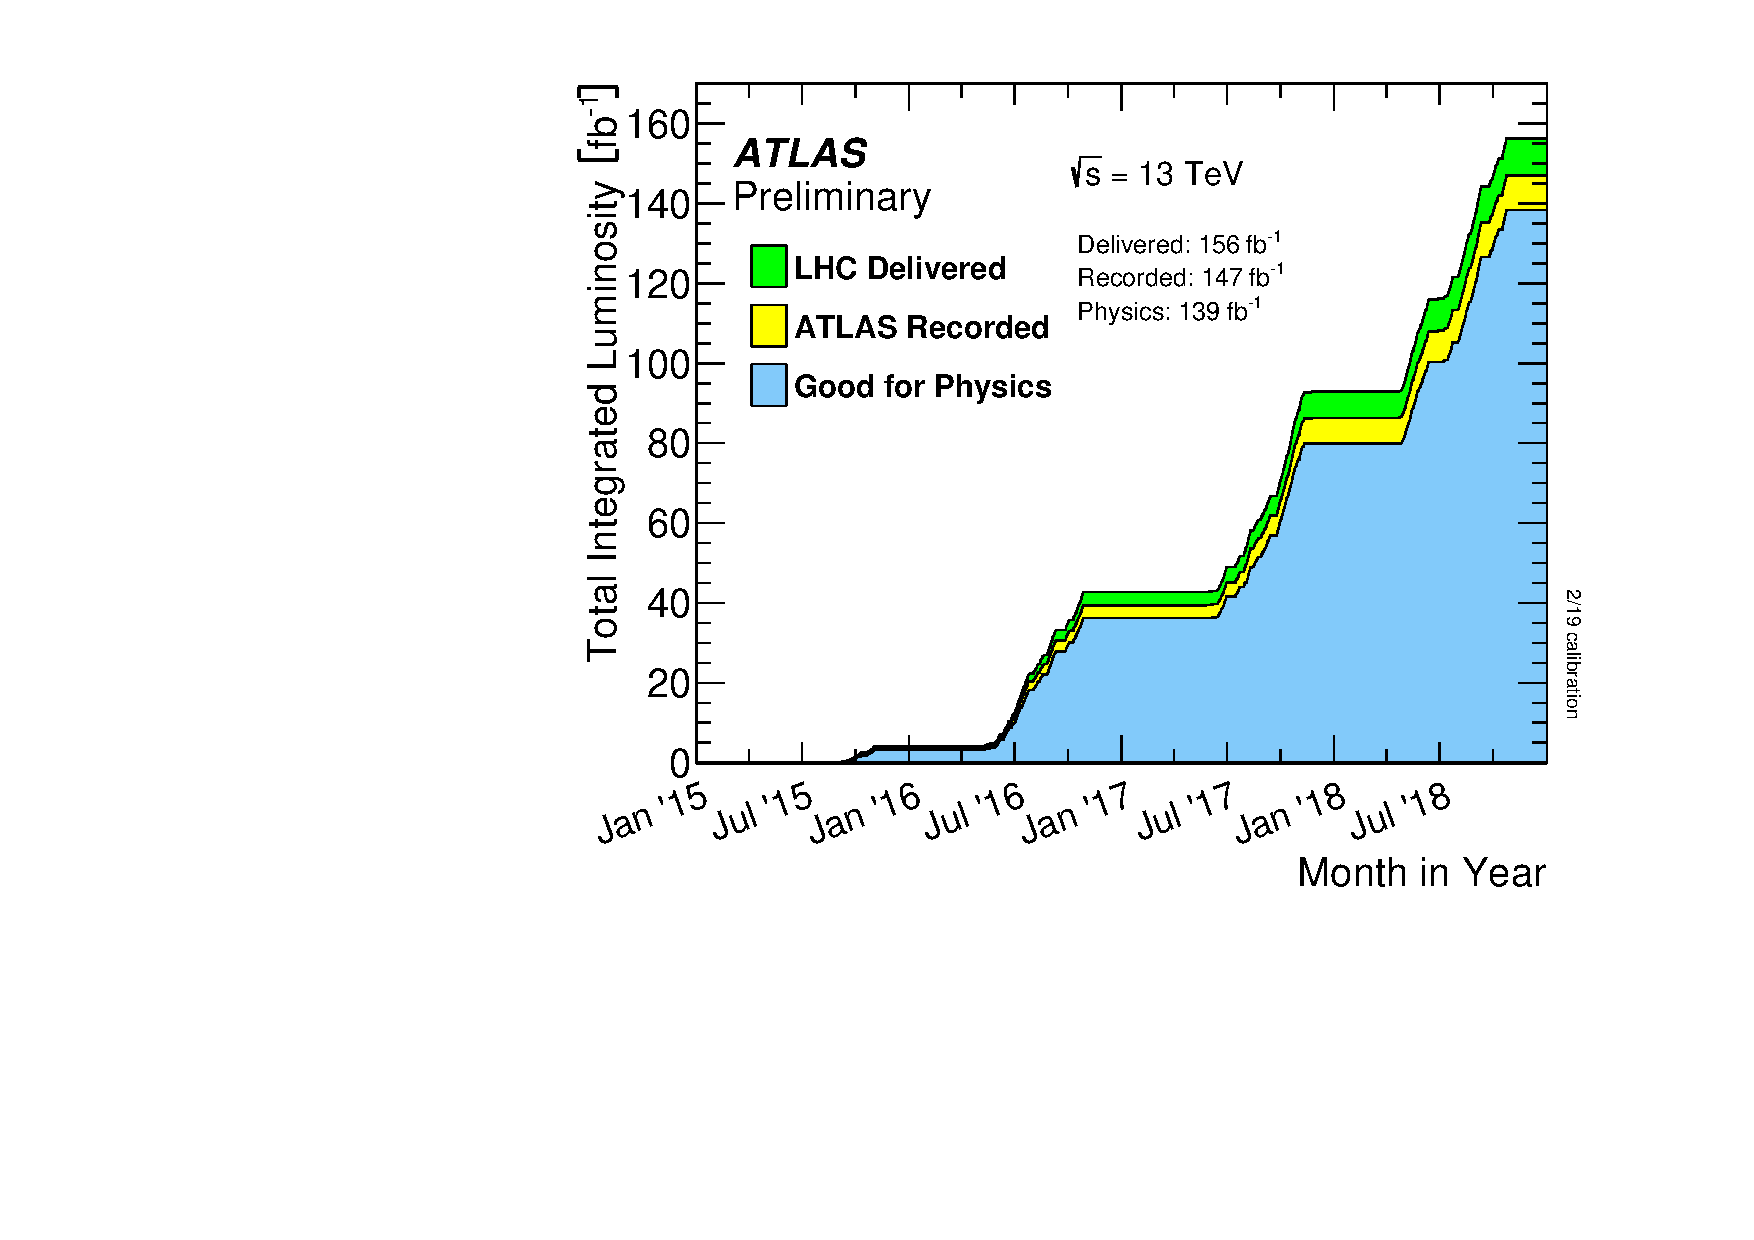
\includegraphics[width=0.6\textwidth]{figures/Detector/intlumivstimeRun2DQall.pdf}
  \caption{Integrated luminosity in ATLAS.}
  \label{fig:lumi_vs_time}
\end{figure}

\textbf{Pile-up}

In collisions, multiple interactions can happen in one single bunch crossing, which is called ``\textit{pile-up}".
The variable $\left< \mu \right>$, representing the average number of interactions per bunch crossing, 
is defined to describe pile-up effect:
\begin{equation}
	\left< \mu \right> = \frac{L_{tot}\sigma}{f_{r}n_{bunch}}
\end{equation}
where $L_{tot}$ is the instantaneous luminosity, $\sigma$ is the inelastic cross section,
$f_{r}$ is the LHC revolution frequency and $n_{bunch}$ is the number of colliding bunches.
Normally, with increasing luminosity, the pile-up becomes more significant.
Figure~\ref{fig:run2_mu} shows the luminosity-weighted distribution of the mean number of interactions per crossing
for pp collision data from 2015 to 2018 (full run-2), the challenge of pile-up increased in each year.
\begin{figure}[!htb]
  \centering
  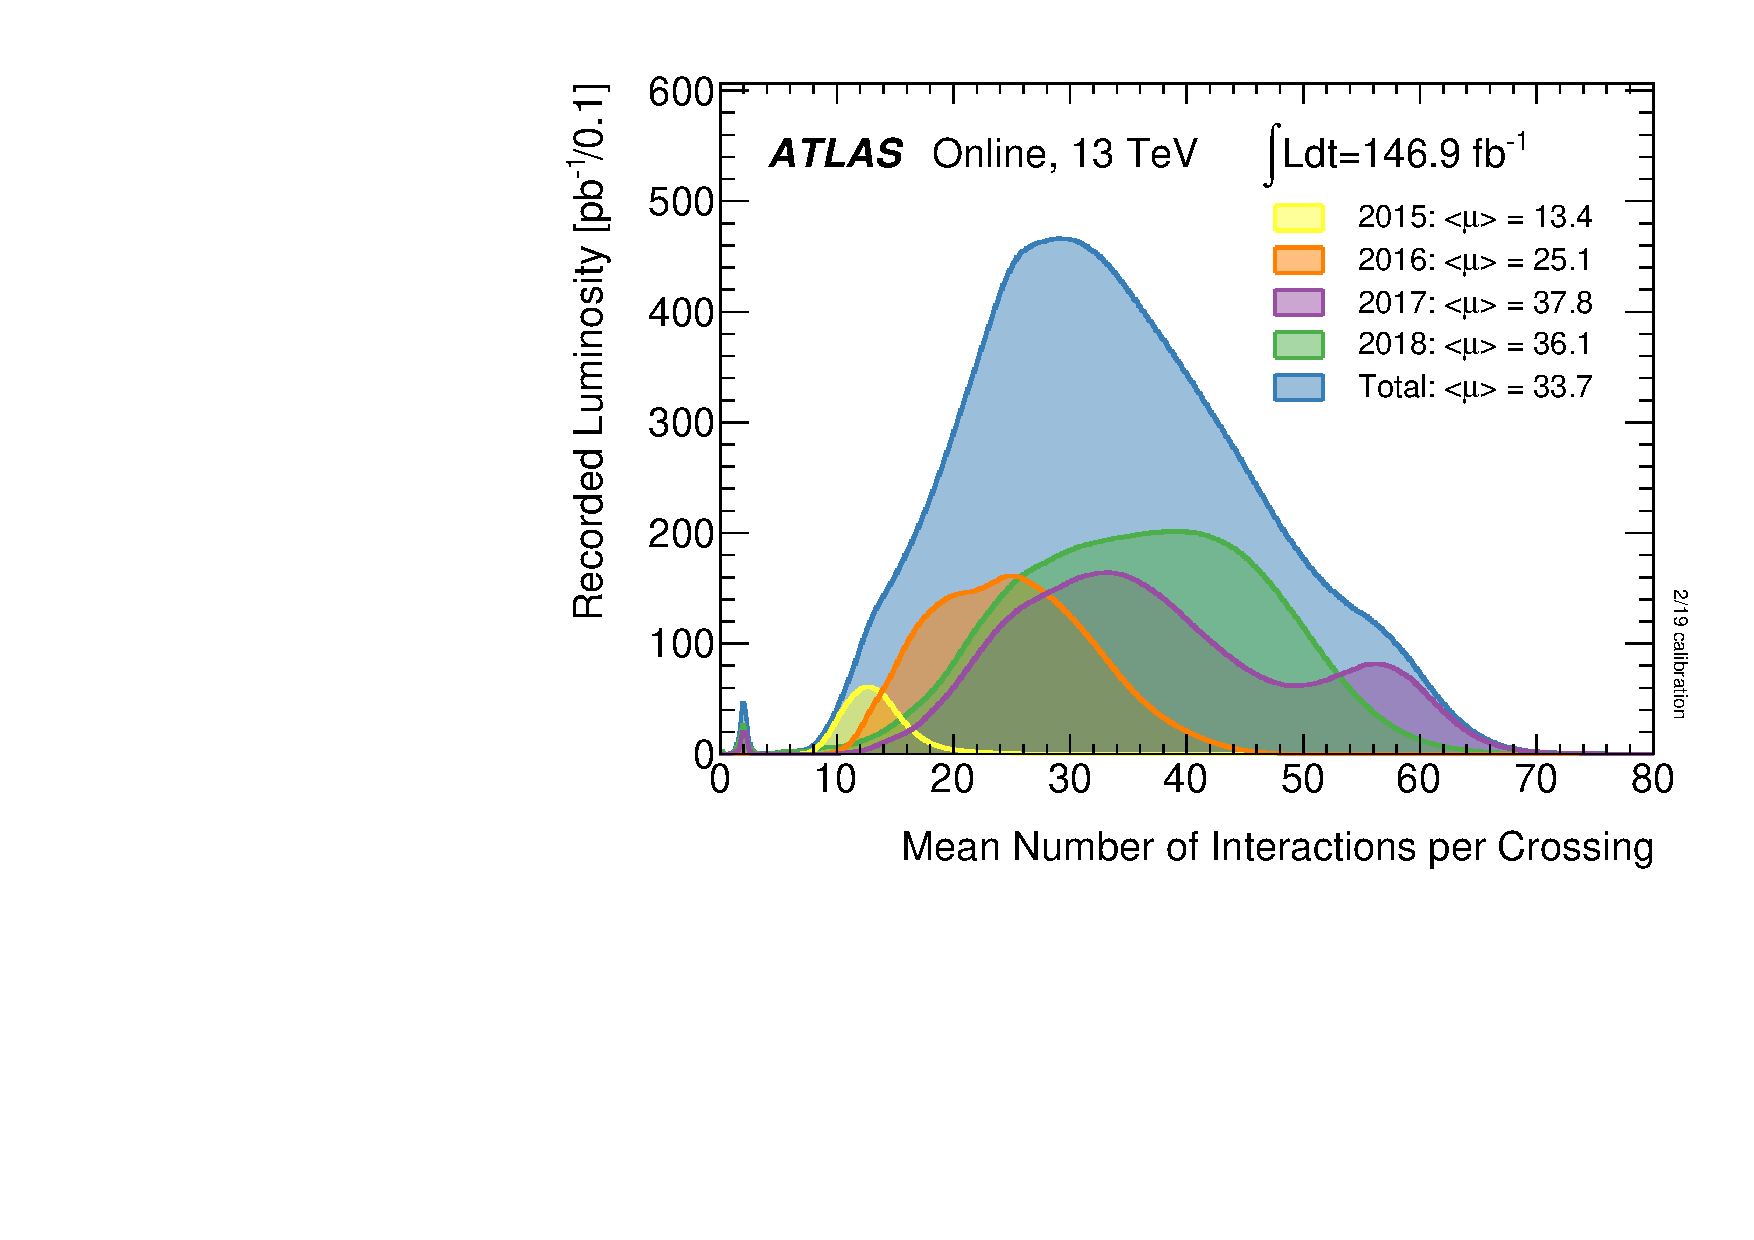
\includegraphics[width=0.6\textwidth]{figures/Detector/mu_2015_2018.pdf}
  \caption{Number of Interactions per Crossing from 2015-2018 in ATLAS.}
  \label{fig:run2_mu}
\end{figure}
